\documentclass[12pt,a4paper]{report}

\usepackage[a4paper,top=2.5cm,bottom=2.5cm,left=3cm,right=2cm]{geometry}
\usepackage{fontspec}
\IfFontExistsTF{Times New Roman}{\setmainfont{Times New Roman}}{\setmainfont{Latin Modern Roman}}
\usepackage{setspace}
\onehalfspacing
\usepackage{indentfirst}
\setlength{\parindent}{1.25cm}
\setlength{\parskip}{0.15cm}
\usepackage{graphicx}
\usepackage{float}
\usepackage{booktabs}
\usepackage{longtable}
\usepackage{tabularx}
\usepackage{array}
\usepackage{ragged2e}
\usepackage{multirow}
\usepackage{enumitem}
\usepackage{xcolor}
\usepackage{listings}
\usepackage{tikz}
\usetikzlibrary{arrows.meta,positioning,shapes.geometric,fit,calc}
\usepackage{hyperref}
\hypersetup{
    colorlinks=true,
    linkcolor=blue!60!black,
    urlcolor=blue!60!black,
    citecolor=blue!60!black
}
\usepackage{caption}
\captionsetup{font=small,labelfont=bf}
\setlength{\emergencystretch}{2em}
\newcolumntype{Y}{>{\RaggedRight\arraybackslash}X}

% ====== Việt hóa nhãn tự động ======
\renewcommand{\contentsname}{Mục lục}
\renewcommand{\listfigurename}{Danh mục hình vẽ}
\renewcommand{\listtablename}{Danh mục bảng biểu}
\renewcommand{\chaptername}{Chương}
\renewcommand{\figurename}{Hình}
\renewcommand{\tablename}{Bảng}
\renewcommand{\lstlistingname}{Mã nguồn}
\renewcommand{\lstlistlistingname}{Danh mục mã nguồn}

\definecolor{codebg}{RGB}{248,248,248}
\definecolor{soccyan}{RGB}{0,180,216}
\definecolor{socpurple}{RGB}{124,58,237}
\definecolor{socgreen}{RGB}{16,185,129}
\definecolor{socred}{RGB}{225,29,72}

\lstdefinestyle{jsonstyle}{
    backgroundcolor=\color{codebg},
    basicstyle=\ttfamily\small,
    frame=single,
    breaklines=true,
    columns=fullflexible,
    showstringspaces=false,
    keepspaces=true,
    tabsize=2
}
\lstset{style=jsonstyle}

% ====== Thông tin cần cập nhật trước khi nộp ======
\newcommand{\ProjectTitle}{SOC AI Search}
\newcommand{\ProjectSubtitle}{Natural Language Search for Security Events}
\newcommand{\StudentName}{<Tên sinh viên thực hiện>}
\newcommand{\StudentEmail}{<Email sinh viên thực hiện>}
\newcommand{\MentorName}{<Tên mentor>}
\newcommand{\UnitName}{<Tên đơn vị>}
\newcommand{\ProgramName}{Viettel Digital Talent 2026}
\newcommand{\TrackName}{Software Engineer}

\begin{document}

\begin{titlepage}
    \begin{center}
        {\bfseries TẬP ĐOÀN CÔNG NGHIỆP -- VIỄN THÔNG QUÂN ĐỘI}\\[0.5cm]
        {\bfseries \Large BÁO CÁO MINI-PROJECT}\\[2.0cm]

        {\bfseries \LARGE \ProjectTitle}\\[0.3cm]
        {\Large \ProjectSubtitle}\\[2.0cm]

        \begin{tabular}{>{\bfseries}p{5cm}p{8cm}}
            Sinh viên thực hiện: & \StudentName \\
            Email: & \StudentEmail \\
            Chương trình: & \ProgramName \\
            Lĩnh vực: & \TrackName \\
            Mentor: & \MentorName \\
            Đơn vị: & \UnitName \\
        \end{tabular}

        \vfill
        {\bfseries Hà Nội, 2026}
    \end{center}
\end{titlepage}

\pagenumbering{roman}

\chapter*{Lời mở đầu}
\addcontentsline{toc}{chapter}{Lời mở đầu}

Trong các trung tâm vận hành an toàn thông tin (Security Operations Center -- SOC), khối lượng log và cảnh báo cần phân tích tăng nhanh theo quy mô hệ thống. Analyst phải thường xuyên trả lời các câu hỏi như ``có bao nhiêu đăng nhập thất bại từ một quốc gia trong 24 giờ qua'', ``top IP nào tạo nhiều cảnh báo nhất'', hoặc ``xu hướng failed login theo giờ như thế nào''. Với các hệ thống tìm kiếm như Elasticsearch, các câu hỏi này thường phải được chuyển thành Query DSL hoặc aggregation DSL. Việc viết DSL thủ công không chỉ mất thời gian mà còn dễ sai, đặc biệt với người mới hoặc trong các tình huống cần phản ứng nhanh.

Đề tài \ProjectTitle{} được xây dựng để giải quyết vấn đề trên theo hướng sử dụng mô hình ngôn ngữ lớn (Large Language Model -- LLM) như một trợ lý tạo kế hoạch truy vấn, nhưng không trao quyền thực thi trực tiếp cho AI. Người dùng đặt câu hỏi bằng tiếng Anh hoặc tiếng Việt; LLM chỉ được phép sinh ra một cấu trúc trung gian có kiểm soát gọi là \texttt{SearchPlan}; backend sau đó parse, validate, compile thành Elasticsearch DSL và thực thi. Cách tiếp cận này giữ được sự tiện lợi của natural language search nhưng vẫn đảm bảo guardrail về bảo mật, kiểm toán và khả năng giải thích.

Báo cáo này trình bày bối cảnh, mục tiêu, kiến trúc, phương pháp triển khai, kết quả đạt được và các hướng phát triển tiếp theo của hệ thống. Nội dung tập trung vào các phần cốt lõi: pipeline Natural Language $\rightarrow$ SearchPlan $\rightarrow$ DSL, guardrail AI, search/aggregation, audit/history, CSV export, RBAC bằng Keycloak, giao diện SOC dashboard và triển khai thực tế trên DigitalOcean với Caddy HTTPS.

\chapter*{Tóm tắt nội dung và đóng góp}
\addcontentsline{toc}{chapter}{Tóm tắt nội dung và đóng góp}

Mini-project \ProjectTitle{} là một hệ thống hỗ trợ SOC analyst tìm kiếm, thống kê và điều tra log bảo mật bằng ngôn ngữ tự nhiên. Hệ thống gồm frontend React/TypeScript, backend Spring Boot, Elasticsearch làm event store, PostgreSQL làm audit/history store, Keycloak làm identity provider, cùng LLM provider dạng mock hoặc Gemini. Sản phẩm đã được triển khai public trên DigitalOcean VPS, định tuyến domain bằng Name.com và HTTPS tự động qua Caddy.

Các đóng góp chính của đề tài gồm:

\begin{itemize}
    \item Thiết kế contract \texttt{SearchPlan} làm lớp trung gian an toàn giữa câu hỏi tự nhiên và Elasticsearch DSL.
    \item Xây dựng pipeline parse/validate/compile để ngăn LLM sinh DSL tùy ý hoặc truy vấn trực tiếp Elasticsearch.
    \item Hỗ trợ search raw events và aggregation cơ bản gồm \texttt{count}, \texttt{group\_by}, \texttt{top\_n}, \texttt{date\_histogram}.
    \item Cung cấp Query Transparency: frontend hiển thị SearchPlan đã validate và DSL đã compile để người dùng kiểm tra.
    \item Tích hợp audit/history, pin investigation, replay query và export CSV an toàn theo \texttt{query\_id}.
    \item Tích hợp Keycloak OIDC và RBAC với ba vai trò \texttt{SOC\_VIEWER}, \texttt{SOC\_ANALYST}, \texttt{SOC\_ADMIN}.
    \item Xây dựng UI dark theme cho SOC console, dashboard, raw events, aggregation charts và investigation workflow.
    \item Thiết lập CI/CD với GitHub Actions, Docker Compose, smoke test và deploy lên VPS.
\end{itemize}

\tableofcontents
\listoffigures
\listoftables
\clearpage
\pagenumbering{arabic}

\chapter{Giới thiệu}

\section{Bối cảnh thực tế}

Trong môi trường doanh nghiệp, hệ thống thông tin tạo ra lượng lớn log từ nhiều nguồn như Windows authentication, VPN, firewall, endpoint, application gateway và cloud services. SOC analyst cần phát hiện các hành vi bất thường như brute force, account lockout, malware detected, privilege escalation hoặc lưu lượng từ quốc gia rủi ro. Những tác vụ này thường yêu cầu truy vấn theo thời gian, mức độ nghiêm trọng, người dùng, IP, host, loại sự kiện và nội dung message.

Elasticsearch là một công cụ mạnh cho bài toán tìm kiếm log, nhưng Query DSL của Elasticsearch tương đối dài và có nhiều chi tiết kỹ thuật. Ví dụ, để tìm failed login trong 24 giờ qua từ Trung Quốc, analyst cần biết cách viết \texttt{bool.filter}, \texttt{range}, \texttt{terms}, \texttt{track\_total\_hits}, phân trang và sort. Khi chuyển sang thống kê, analyst còn phải nắm thêm \texttt{terms aggregation} hoặc \texttt{date\_histogram}. Đây là rào cản lớn cho tốc độ điều tra và khả năng onboarding thành viên mới.

LLM có thể giúp chuyển câu hỏi tự nhiên thành truy vấn. Tuy nhiên, nếu cho LLM sinh Elasticsearch DSL trực tiếp rồi execute ngay, hệ thống sẽ đối mặt với nhiều rủi ro: sinh field không tồn tại, query quá lớn, script/wildcard/query string không kiểm soát, hoặc bypass cơ chế audit/RBAC. Vì vậy, đề tài chọn hướng ``AI hỗ trợ, backend kiểm soát''.

\section{Mục tiêu đề tài}

Mục tiêu tổng quát của đề tài là xây dựng một MVP cho phép SOC analyst hỏi bằng ngôn ngữ tự nhiên, nhận kết quả search/aggregation minh bạch, đồng thời đảm bảo an toàn bằng validator, compiler, RBAC và audit.

Các mục tiêu cụ thể:

\begin{enumerate}
    \item Cho phép người dùng đặt câu hỏi bằng tiếng Anh hoặc tiếng Việt.
    \item Chuyển câu hỏi thành \texttt{SearchPlan} JSON thay vì DSL trực tiếp.
    \item Validate chặt chẽ \texttt{SearchPlan}: mode, filter, aggregation type, allowlist field, pagination và bucket limit.
    \item Compile \texttt{SearchPlan} thành Elasticsearch DSL bằng backend.
    \item Hiển thị kết quả raw events hoặc aggregation charts trên giao diện SOC.
    \item Lưu query history/audit vào PostgreSQL để replay, pin, export và truy vết.
    \item Bảo vệ các chức năng bằng Keycloak OIDC và RBAC.
    \item Triển khai hệ thống chạy thật trên VPS với domain và HTTPS.
\end{enumerate}

\section{Phạm vi triển khai}

Phạm vi MVP tập trung vào dữ liệu synthetic SOC events với schema cố định. Elasticsearch lưu toàn bộ event documents, trong khi PostgreSQL chỉ lưu metadata như audit, history, SearchPlan, DSL, summary và thông tin export replay.

Hệ thống hiện hỗ trợ hai chế độ truy vấn:

\begin{itemize}
    \item \textbf{Search mode}: trả danh sách raw events có phân trang.
    \item \textbf{Aggregation mode}: trả kết quả thống kê chuẩn hóa để frontend render chart.
\end{itemize}

Các tính năng nằm ngoài phạm vi MVP gồm multi-turn chat, vector search, anomaly detection production-grade, multi-tenant enterprise, Kubernetes và streaming realtime quy mô lớn.

\section{Đóng góp của mini-project}

Đóng góp quan trọng nhất của đề tài không chỉ là gọi LLM để tạo query, mà là thiết kế một pipeline có guardrail:

\begin{center}
\textbf{Natural Language $\rightarrow$ SearchPlan $\rightarrow$ Validator $\rightarrow$ Compiler $\rightarrow$ Elasticsearch}
\end{center}

LLM không được truy vấn dữ liệu trực tiếp. Frontend không được gửi DSL tùy ý. Người dùng có thể xem SearchPlan và DSL để hiểu hệ thống đã diễn dịch câu hỏi như thế nào. Đây là yếu tố quan trọng với một hệ thống SOC, nơi tính minh bạch và truy vết thường quan trọng không kém tính tiện dụng.

\chapter{Nội dung và phương pháp}

\section{Tổng quan kiến trúc hệ thống}

Hệ thống được thiết kế theo mô hình modular monolith ở backend. Backend Spring Boot chứa các module search, LLM, validation, compiler, execution, summary, audit, CSV export, event detail và security. Frontend là React SPA độc lập. Các thành phần hạ tầng gồm Elasticsearch, PostgreSQL, Keycloak và Caddy.

\begin{figure}[H]
\centering
\resizebox{0.98\textwidth}{!}{%
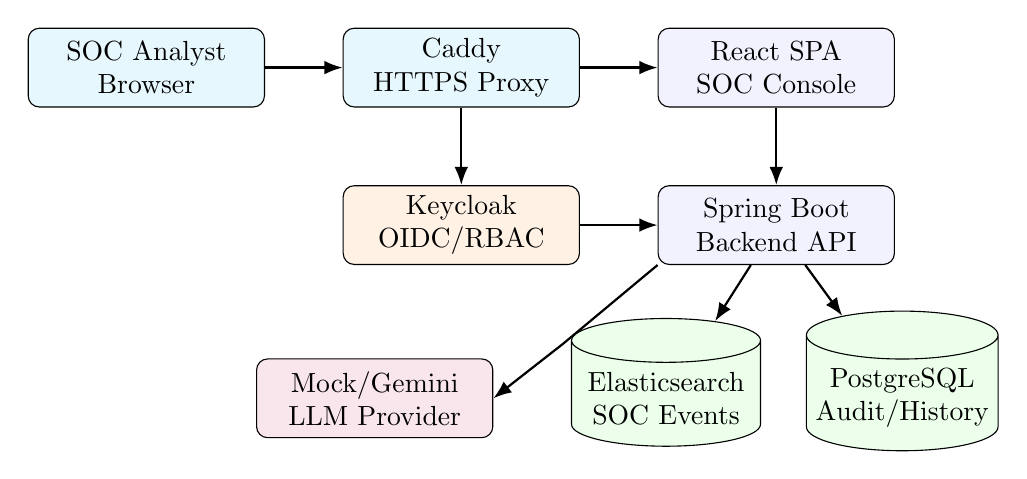
\begin{tikzpicture}[
    box/.style={draw, rounded corners, minimum width=3.0cm, minimum height=1.0cm, align=center, fill=blue!5},
    store/.style={draw, cylinder, shape border rotate=90, aspect=0.25, minimum width=2.4cm, minimum height=1.1cm, align=center, fill=green!8},
    arrow/.style={-Latex, thick}
]
\node[box, fill=cyan!10] (user) at (0,0) {SOC Analyst\\Browser};
\node[box, fill=cyan!10] (caddy) at (4,0) {Caddy\\HTTPS Proxy};
\node[box] (fe) at (8,0) {React SPA\\SOC Console};
\node[box, fill=orange!10] (kc) at (4,-2.0) {Keycloak\\OIDC/RBAC};
\node[box] (be) at (8,-2.0) {Spring Boot\\Backend API};
\node[box, fill=purple!10] (llm) at (2.9,-4.2) {Mock/Gemini\\LLM Provider};
\node[store] (es) at (6.6,-4.2) {Elasticsearch\\SOC Events};
\node[store] (pg) at (9.6,-4.2) {PostgreSQL\\Audit/History};

\draw[arrow] (user) -- (caddy);
\draw[arrow] (caddy) -- (fe);
\draw[arrow] (caddy) -- (kc);
\draw[arrow] (fe) -- (be);
\draw[arrow] (kc) -- (be);
\draw[arrow] (be.south west) -- ++(-1.2,-1.0) -- (llm.east);
\draw[arrow] (be) -- (es);
\draw[arrow] (be) -- (pg);
\end{tikzpicture}
}
\caption{Kiến trúc tổng quan của SOC AI Search}
\label{fig:architecture}
\end{figure}

Trong kiến trúc này, frontend không kết nối trực tiếp đến Elasticsearch, PostgreSQL hoặc LLM. Tất cả request nghiệp vụ đi qua backend. Điều này giúp tập trung enforcement tại một nơi: JWT/RBAC, validation, compiler, audit và error handling.

\section{Công nghệ sử dụng}

\begin{longtable}{p{4cm}p{10cm}}
\caption{Technology stack của hệ thống}\\
\toprule
\textbf{Nhóm} & \textbf{Công nghệ và vai trò} \\
\midrule
\endfirsthead
\toprule
\textbf{Nhóm} & \textbf{Công nghệ và vai trò} \\
\midrule
\endhead
Frontend & React, TypeScript, Vite, Tailwind CSS, shadcn/ui, lucide-react, Recharts. Dùng để xây dựng SOC console, dashboard, bảng raw events, biểu đồ aggregation và trang investigations. \\
Backend & Java 21, Spring Boot 3, Spring Security, Spring Web, Bean Validation, Jackson, springdoc-openapi. Dùng để triển khai API, pipeline xử lý SearchPlan, RBAC và Swagger. \\
Search engine & Elasticsearch 9.4.2. Lưu SOC events, thực thi query, filter, full-text search và aggregation. \\
Database metadata & PostgreSQL 17. Lưu audit logs, query history, SearchPlan, generated DSL, summary và dữ liệu phục vụ replay/export. \\
Authentication & Keycloak. Cung cấp OIDC, JWT, realm roles và user onboarding. \\
LLM & Mock provider cho local/test/CI và Google Gemini cho demo AI thật. \\
Deployment & Docker Compose, Caddy, DigitalOcean VPS, Name.com DNS. \\
CI/CD & GitHub Actions, backend tests, frontend tests/build, compose validation, SSH deploy và smoke test domain. \\
\bottomrule
\end{longtable}

\section{Mô hình dữ liệu sự kiện}

Elasticsearch index \texttt{soc-events-v1} lưu các event bảo mật. Schema MVP được giữ cố định để compiler có thể sinh DSL an toàn và validator có thể allowlist field.

\begin{table}[H]
\centering
\caption{Schema chính của SOC event}
\begin{tabular}{p{4cm}p{4cm}p{6cm}}
\toprule
\textbf{Field} & \textbf{Kiểu trong Elasticsearch} & \textbf{Ý nghĩa} \\
\midrule
\texttt{timestamp} & date & Thời điểm xảy ra event. \\
\texttt{source} & keyword & Nguồn log như windows-auth, vpn, firewall. \\
\texttt{severity} & keyword & Mức độ: low, medium, high, critical. \\
\texttt{event\_type} & keyword & Loại sự kiện: failed\_login, malware\_detected, account\_lockout, v.v. \\
\texttt{user} & keyword & Tài khoản liên quan. \\
\texttt{host} & keyword & Host hoặc thiết bị liên quan. \\
\texttt{ip} & ip & IP nguồn/đích trong event. \\
\texttt{country\_code} & keyword & Mã quốc gia như CN, US, VN. \\
\texttt{message} & text & Nội dung mô tả event, hỗ trợ full-text search. \\
\texttt{raw} & text, index=false & Raw log phục vụ forensic detail. \\
\bottomrule
\end{tabular}
\end{table}

Dữ liệu demo được seed bằng PowerShell scripts. PostgreSQL không lưu raw events; nguyên tắc này giúp tách bạch event store và metadata store.

\section{Pipeline Natural Language Search}

Pipeline Natural Language Search là phần cốt lõi của đề tài. Người dùng nhập câu hỏi, backend gọi LLM để sinh \texttt{SearchPlan}, sau đó backend kiểm soát toàn bộ phần còn lại.

\begin{figure}[H]
\centering
\resizebox{0.98\textwidth}{!}{%
\begin{tikzpicture}[
    node distance=0.9cm,
    flowstep/.style={draw, rounded corners, minimum width=10.5cm, minimum height=0.8cm, align=center, fill=gray!8},
    arrow/.style={-Latex, thick}
]
\node[flowstep, fill=cyan!10] (s1) {1. Frontend gửi \texttt{POST /api/v1/search}: question, page, size};
\node[flowstep, below=of s1] (s2) {2. Backend build prompt bằng \texttt{SearchPlanPromptBuilder}};
\node[flowstep, below=of s2, fill=purple!8] (s3) {3. \texttt{LlmClient}: mock hoặc Gemini trả raw SearchPlan JSON};
\node[flowstep, below=of s3] (s4) {4. \texttt{SearchPlanJsonParser}: parse JSON thuần, reject markdown/prose/unknown field};
\node[flowstep, below=of s4] (s5) {5. \texttt{SearchPlanValidator}: validate rule search/aggregation};
\node[flowstep, below=of s5] (s6) {6. Backend override page/size từ request};
\node[flowstep, below=of s6] (s7) {7. \texttt{SearchPlanCompiler}: sinh Elasticsearch DSL};
\node[flowstep, below=of s7] (s8) {8. Executor gọi Elasticsearch, mapper chuẩn hóa response};
\node[flowstep, below=of s8, fill=green!8] (s9) {9. Lưu audit/history, trả response gồm SearchPlan, DSL, kết quả};
\foreach \a/\b in {s1/s2,s2/s3,s3/s4,s4/s5,s5/s6,s6/s7,s7/s8,s8/s9} {
    \draw[arrow] (\a) -- (\b);
}
\end{tikzpicture}
}
\caption{Pipeline Natural Language Search}
\label{fig:nl-pipeline}
\end{figure}

Ví dụ một \texttt{SearchPlan} hợp lệ:

\begin{lstlisting}[caption={Ví dụ SearchPlan cho câu hỏi failed login từ China}]
{
  "mode": "search",
  "filters": {
    "timestamp": {
      "from": "now-24h",
      "to": "now"
    },
    "event_type": ["failed_login"],
    "country_code": ["CN"]
  },
  "page": 0,
  "size": 10
}
\end{lstlisting}

\section{Tích hợp LLM: Mock và Gemini}

Hệ thống không tự train model. Backend định nghĩa interface \texttt{LlmClient} để trừu tượng hóa provider. Hiện có hai provider:

\begin{itemize}
    \item \textbf{Mock}: trả về SearchPlan deterministic cho các câu demo/regression test. Provider này không cần API key, không gọi mạng và phù hợp cho local development, CI, smoke test.
    \item \textbf{Gemini}: gọi Google Gemini REST API bằng cấu hình runtime như provider, base URL, API key và model. Các biến cấu hình tương ứng là \texttt{LLM\_PROVIDER}, \texttt{LLM\_BASE\_URL}, \texttt{LLM\_API\_KEY} và \texttt{LLM\_MODEL}.
\end{itemize}

Gemini client chỉ chịu trách nhiệm gọi API và trích text từ response. Việc parse SearchPlan, validate rule và compile DSL hoàn toàn nằm trong backend service khác. Đây là điểm quan trọng để tránh trộn logic AI với logic thực thi.

\begin{figure}[H]
\centering
\resizebox{0.98\textwidth}{!}{%
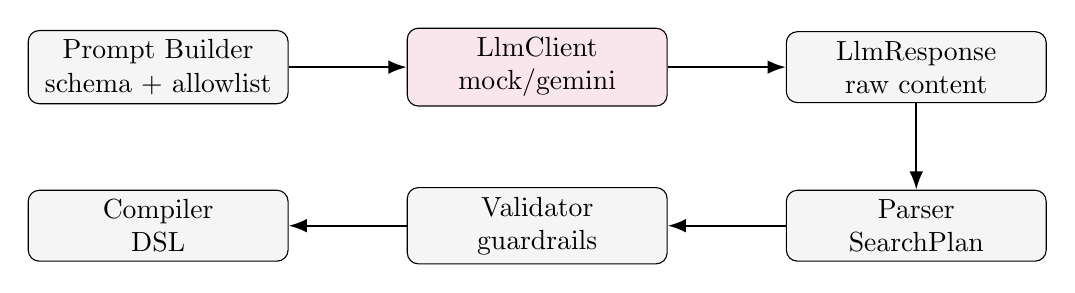
\begin{tikzpicture}[
    node distance=1.1cm and 1.5cm,
    box/.style={draw, rounded corners, minimum width=3.3cm, minimum height=0.9cm, align=center, fill=gray!8},
    arrow/.style={-Latex, thick}
]
\node[box] (prompt) {Prompt Builder\\schema + allowlist};
\node[box, right=of prompt, fill=purple!10] (llm) {LlmClient\\mock/gemini};
\node[box, right=of llm] (resp) {LlmResponse\\raw content};
\node[box, below=of resp] (parser) {Parser\\SearchPlan};
\node[box, left=of parser] (validator) {Validator\\guardrails};
\node[box, left=of validator] (compiler) {Compiler\\DSL};
\draw[arrow] (prompt) -- (llm);
\draw[arrow] (llm) -- (resp);
\draw[arrow] (resp) -- (parser);
\draw[arrow] (parser) -- (validator);
\draw[arrow] (validator) -- (compiler);
\end{tikzpicture}
}
\caption{Tách biệt LLM provider khỏi parser/validator/compiler}
\label{fig:llm}
\end{figure}

\section{SearchPlan: contract trung gian an toàn}

\texttt{SearchPlan} là biểu diễn nghiệp vụ có cấu trúc, dễ hiểu hơn DSL nhưng đủ chặt để backend validate. Contract này gồm:

\begin{itemize}
    \item \texttt{mode}: \texttt{search} hoặc \texttt{aggregation}.
    \item \texttt{filters}: time range, severity, event type, user, host, ip, country code, message query.
    \item \texttt{page}, \texttt{size}: pagination contract.
    \item \texttt{aggregation}: optional, dùng khi mode là aggregation.
\end{itemize}

SearchPlan không chứa Elasticsearch-specific DSL field như \texttt{query}, \texttt{aggs}, \texttt{script}, \texttt{wildcard}. Nếu LLM hoặc user thêm các field này, parser/validator sẽ reject trước khi compiler sinh DSL.

\section{Validation và guardrails}

Guardrail của hệ thống được đặt ở nhiều lớp:

\begin{enumerate}
    \item \textbf{Prompt constraint}: yêu cầu LLM chỉ trả JSON SearchPlan thuần, không markdown, không prose, không DSL.
    \item \textbf{Jackson strict parser}: reject unknown fields và output không phải JSON object.
    \item \textbf{Bean Validation}: validate field cơ bản như question not blank, page/size range.
    \item \textbf{SearchPlanValidator}: validate rule nghiệp vụ: mode, aggregation type, allowlist field, top\_n, interval, message\_query trong aggregation.
    \item \textbf{Compiler ownership}: chỉ backend compiler được sinh DSL.
    \item \textbf{RBAC}: backend kiểm tra quyền thao tác như edit SearchPlan, export CSV, xem audit logs.
\end{enumerate}

\begin{table}[H]
\centering
\caption{Một số rule validation quan trọng}
\begin{tabularx}{\textwidth}{p{4.2cm}Y}
\toprule
\textbf{Rule} & \textbf{Mục đích} \\
\midrule
Reject unknown fields & Ngăn LLM/user thêm field ngoài schema. \\
Backend override page/size & Ngăn LLM tự tăng size hoặc đổi page ngoài request. \\
Aggregation field allowlist & Chỉ cho phép source, severity, event\_type, user, host, ip, country\_code. \\
Reject \texttt{.keyword} & Mapping MVP đã định nghĩa keyword trực tiếp; không để LLM tự gắn field Elasticsearch-specific. \\
Reject \texttt{script}, \texttt{wildcard}, \texttt{query\_string} & Giảm nguy cơ query nguy hiểm hoặc tốn tài nguyên. \\
Repair tối đa một lần & Có khả năng tự sửa lỗi nhẹ nhưng tránh retry loop vô hạn. \\
\bottomrule
\end{tabularx}
\end{table}

\section{Compiler và Elasticsearch DSL}

\texttt{SearchPlanCompiler} nhận một SearchPlan đã validate và sinh Java structure tương thích với Elasticsearch request. Compiler không build JSON bằng nối chuỗi thủ công mà dùng cấu trúc \texttt{Map<String,Object>} hoặc object nội bộ.

Với search mode, compiler sinh \texttt{bool.filter} gồm range, terms, term và match phù hợp. Mặc định sort theo \texttt{timestamp desc}. Với aggregation mode, compiler sinh DSL theo loại aggregation:

\begin{table}[H]
\centering
\caption{Mapping aggregation sang Elasticsearch DSL}
\small
\begin{tabularx}{\textwidth}{p{2.8cm}p{4.0cm}Y}
\toprule
\textbf{Aggregation} & \textbf{DSL chính} & \textbf{Ghi chú} \\
\midrule
\texttt{count} & \texttt{size = 0}, không có \texttt{aggs} & Lấy \texttt{hits.total}. \\
\texttt{group\_by} & \texttt{terms} aggregation & Nếu thiếu \texttt{top\_n}, default bucket limit = 20. \\
\texttt{top\_n} & \texttt{terms} aggregation & Bắt buộc \texttt{top\_n} từ 1 đến 100. \\
\texttt{date\_histogram} & \texttt{date\_histogram} trên \texttt{timestamp} & Dùng \texttt{fixed\_interval}: minute = 1m, hour = 1h, day = 1d. \\
\bottomrule
\end{tabularx}
\end{table}

Generated DSL được trả về response dưới dạng object/map, không phải JSON string escaped. Điều này giúp frontend render pretty JSON trong Query Transparency panel.

\section{Search và Aggregation response}

Search response trả về raw events, pagination, summary và telemetry:

\begin{lstlisting}[caption={Schema rút gọn của natural language search response}]
{
  "query_id": "uuid",
  "original_question": "...",
  "mode": "search",
  "search_plan": {},
  "generated_dsl": {},
  "summary": "...",
  "summary_source": "llm",
  "total": 178,
  "page": 0,
  "size": 10,
  "events": []
}
\end{lstlisting}

Aggregation response không trả event list thật; \texttt{events} là mảng rỗng để frontend xử lý nhất quán. Kết quả chính nằm ở \texttt{aggregation\_results} và \texttt{chart\_metadata}.

\begin{lstlisting}[caption={Schema rút gọn của aggregation response}]
{
  "mode": "aggregation",
  "aggregation_type": "top_n",
  "aggregation_results": [
    { "key": "203.0.113.45", "value": 124 }
  ],
  "chart_metadata": {
    "chart_type": "BAR",
    "x_axis_label": "ip",
    "y_axis_label": "count"
  },
  "events": []
}
\end{lstlisting}

\section{AI summary best-effort}

AI summary giúp analyst đọc nhanh kết quả. Tuy nhiên, summary không được làm hỏng request search. Vì vậy hệ thống áp dụng nguyên tắc best-effort:

\begin{itemize}
    \item Search result/aggregation result luôn được ưu tiên trả về.
    \item Nếu LLM timeout hoặc trả summary không hợp lệ, backend dùng deterministic fallback.
    \item Payload gửi cho LLM được giới hạn: không gửi raw log đầy đủ, không gửi toàn bộ event documents.
    \item Với aggregation mode, summary dùng trực tiếp \texttt{aggregation\_results}; không query Elasticsearch thêm lần nữa.
\end{itemize}

Nguyên tắc này giúp trải nghiệm người dùng ổn định hơn, đồng thời tránh chi phí và rủi ro gửi dữ liệu nhạy cảm ra ngoài.

\section{Audit, history và investigation workflow}

Mỗi truy vấn được lưu vào PostgreSQL trong bảng \texttt{search\_query\_logs}. Bảng này phục vụ ba mục tiêu:

\begin{enumerate}
    \item \textbf{Audit}: biết ai đã query gì, lúc nào, mode nào, status ra sao.
    \item \textbf{History}: hiển thị Recent Queries và All Investigations trên UI.
    \item \textbf{Replay}: dùng \texttt{query\_id} để chạy lại query hoặc export CSV.
\end{enumerate}

Các trường chính gồm query id, identity, question, mode, status, failure stage, SearchPlan, generated DSL, result count, latency, summary, error message và created time. Việc lưu SearchPlan/DSL giúp analyst có thể truy vết câu hỏi tự nhiên đã được chuyển thành logic kỹ thuật như thế nào.

\section{CSV export an toàn}

CSV export không nhận DSL tùy ý từ client. Thay vào đó, frontend chỉ gửi \texttt{query\_id}. Backend load SearchPlan đã lưu từ PostgreSQL, kiểm tra quyền truy cập, validate lại, compile lại DSL và replay trên Elasticsearch. Kết quả export có giới hạn tối đa 10.000 dòng.

\begin{figure}[H]
\centering
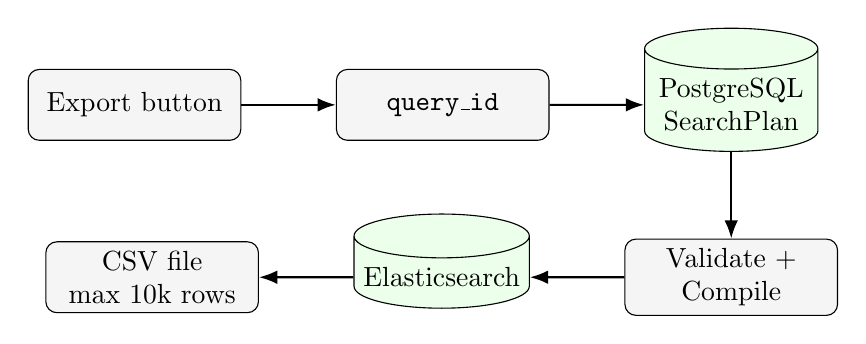
\begin{tikzpicture}[
    node distance=1.1cm and 1.2cm,
    box/.style={draw, rounded corners, minimum width=2.7cm, minimum height=0.9cm, align=center, fill=gray!8},
    store/.style={draw, cylinder, shape border rotate=90, aspect=0.25, minimum width=2.2cm, minimum height=1.0cm, align=center, fill=green!8},
    arrow/.style={-Latex, thick}
]
\node[box] (ui) {Export button};
\node[box, right=of ui] (qid) {\texttt{query\_id}};
\node[store, right=of qid] (pg) {PostgreSQL\\SearchPlan};
\node[box, below=of pg] (compiler) {Validate +\\Compile};
\node[store, left=of compiler] (es) {Elasticsearch};
\node[box, left=of es] (csv) {CSV file\\max 10k rows};
\draw[arrow] (ui) -- (qid);
\draw[arrow] (qid) -- (pg);
\draw[arrow] (pg) -- (compiler);
\draw[arrow] (compiler) -- (es);
\draw[arrow] (es) -- (csv);
\end{tikzpicture}
\caption{CSV export theo cơ chế replay SearchPlan}
\label{fig:csv}
\end{figure}

Cách làm này giảm nguy cơ client gửi DSL độc hại và đảm bảo export vẫn đi qua guardrail backend.

\section{Xác thực và phân quyền}

Hệ thống sử dụng Keycloak làm Identity Provider theo chuẩn OIDC. Frontend dùng OIDC flow để lấy access token, sau đó gọi backend bằng Bearer token. Backend là nơi enforce quyền thật sự bằng Spring Security Resource Server.

\begin{table}[H]
\centering
\caption{RBAC matrix của hệ thống}
\begin{tabular}{lccc}
\toprule
\textbf{Chức năng} & \textbf{SOC\_VIEWER} & \textbf{SOC\_ANALYST} & \textbf{SOC\_ADMIN} \\
\midrule
Đăng nhập và xem dashboard & Có & Có & Có \\
Natural language search & Có & Có & Có \\
Xem event detail & Có & Có & Có \\
Edit SearchPlan & Không & Có & Có \\
Pin investigation & Không & Có & Có \\
Export CSV & Không & Có & Có \\
Xem audit logs toàn hệ thống & Không & Không & Có \\
\bottomrule
\end{tabular}
\end{table}

Frontend ẩn/disable các nút không phù hợp để cải thiện UX, nhưng backend vẫn là nguồn kiểm tra quyền cuối cùng. Điều này tránh trường hợp người dùng sửa UI hoặc gọi API thủ công để bypass quyền.

\section{Frontend SOC Console}

Frontend được xây dựng theo dark SOC/SIEM style, tập trung vào khả năng quan sát nhanh và minh bạch truy vấn. Các thành phần chính:

\begin{itemize}
    \item Landing/Auth gateway.
    \item Event Search với suggested queries và query input.
    \item KPI cards: mode, total events, SearchPlan status, LLM latency, execution latency.
    \item AI Summary block.
    \item Query Transparency: SearchPlan và compiled DSL.
    \item Raw Events table, Event Detail Drawer.
    \item Aggregation charts bằng Recharts và summary table.
    \item SOC Overview Dashboard auto-refresh 10 phút.
    \item Recent Queries drawer và All Investigations page.
    \item Admin Audit Logs page.
    \item Trang All Investigations và Audit Logs áp dụng bố cục \textbf{Master-Detail (chia đôi 35/65)} với thanh cuộn độc lập, giúp điều tra log chi tiết mà không làm mất bối cảnh (context) của danh sách tổng.
\end{itemize}

\begin{figure}[H]
\centering
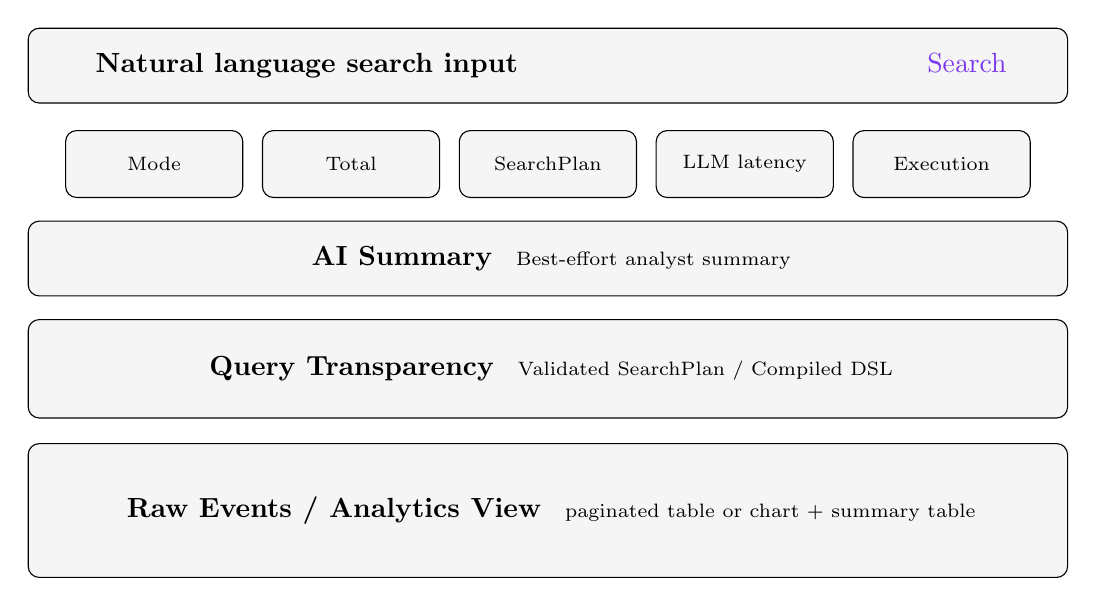
\begin{tikzpicture}[
    panel/.style={draw, rounded corners, fill=black!4, minimum height=0.8cm},
    label/.style={font=\small\bfseries},
    sublabel/.style={font=\scriptsize}
]
\node[panel, minimum width=13.2cm, minimum height=0.95cm, align=left] (search) at (0,0) {
    \hspace{0.2cm}\textbf{Natural language search input}\hspace{5.2cm}\textcolor{socpurple}{Search}
};
\foreach \x/\name in {-5.0/Mode, -2.5/Total, 0/SearchPlan, 2.5/LLM latency, 5.0/Execution} {
    \node[panel, minimum width=2.25cm, minimum height=0.85cm] at (\x,-1.25) {\scriptsize \name};
}
\node[panel, minimum width=13.2cm, minimum height=0.95cm, align=left] at (0,-2.45) {
    \hspace{0.2cm}\textbf{AI Summary}\hspace{0.3cm}{\scriptsize Best-effort analyst summary}
};
\node[panel, minimum width=13.2cm, minimum height=1.25cm, align=left] at (0,-3.85) {
    \hspace{0.2cm}\textbf{Query Transparency}\hspace{0.3cm}{\scriptsize Validated SearchPlan / Compiled DSL}
};
\node[panel, minimum width=13.2cm, minimum height=1.7cm, align=left] at (0,-5.65) {
    \hspace{0.2cm}\textbf{Raw Events / Analytics View}\hspace{0.3cm}{\scriptsize paginated table or chart + summary table}
};
\end{tikzpicture}
\caption{Minh họa bố cục chính của giao diện Event Search}
\label{fig:event-search-placeholder}
\end{figure}

\section{SOC Overview Dashboard và query suggestions}

SOC Overview Dashboard dùng các SearchPlan/aggregation cố định thay vì gọi LLM. Các card tối thiểu gồm Total Events, Failed Logins, Critical Alerts, Severity Distribution, Top Source IPs và Events Over Time. Dashboard auto-refresh mỗi 10 phút để cập nhật dữ liệu mới.

Query suggestions và investigation playbooks tĩnh giúp analyst bắt đầu nhanh với các tình huống như failed login, critical alerts, top source IPs, events by hour. Đây là lựa chọn phù hợp với MVP vì không tốn token LLM, ổn định khi demo và vẫn có giá trị UX.

\section{Triển khai và CI/CD}

Hệ thống được deploy trên DigitalOcean Droplet. Domain được mua và quản lý DNS tại Name.com. Caddy làm reverse proxy và tự động cấp HTTPS cho các domain:

\begin{itemize}
    \item \url{https://soc-ai-search.app}: frontend.
    \item \url{https://api.soc-ai-search.app}: backend API và Swagger.
    \item \url{https://auth.soc-ai-search.app}: Keycloak.
\end{itemize}

Docker Compose chạy các service chính: frontend, backend, Elasticsearch, PostgreSQL, Keycloak và Caddy. GitHub Actions đảm nhiệm CI/CD: test, build, kiểm tra compose config, SSH vào VPS, pull code, rebuild container và chạy smoke test public domain.

\begin{figure}[H]
\centering
\resizebox{0.98\textwidth}{!}{%
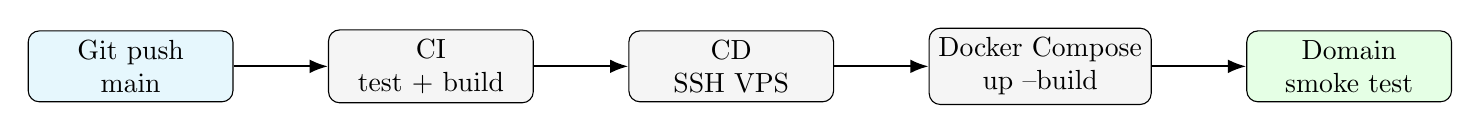
\begin{tikzpicture}[
    node distance=1.2cm and 1.2cm,
    box/.style={draw, rounded corners, minimum width=2.6cm, minimum height=0.9cm, align=center, fill=gray!8},
    arrow/.style={-Latex, thick}
]
\node[box, fill=cyan!10] (push) {Git push\\main};
\node[box, right=of push] (ci) {CI\\test + build};
\node[box, right=of ci] (ssh) {CD\\SSH VPS};
\node[box, right=of ssh] (compose) {Docker Compose\\up --build};
\node[box, right=of compose, fill=green!10] (smoke) {Domain\\smoke test};
\draw[arrow] (push) -- (ci);
\draw[arrow] (ci) -- (ssh);
\draw[arrow] (ssh) -- (compose);
\draw[arrow] (compose) -- (smoke);
\end{tikzpicture}
}
\caption{CI/CD pipeline triển khai lên VPS}
\label{fig:cicd}
\end{figure}

\chapter{Kết quả thực hiện và đánh giá}

\section{Kết quả chức năng}

Hệ thống đã hoàn thành các nhóm chức năng chính của MVP:

\begin{table}[H]
\centering
\caption{Tổng hợp kết quả chức năng đã triển khai}
\begin{tabularx}{\textwidth}{p{3.6cm}Y}
\toprule
\textbf{Nhóm chức năng} & \textbf{Kết quả} \\
\midrule
Natural Language Search & Hỗ trợ câu hỏi tiếng Anh/Việt qua \texttt{POST /api/v1/search}; provider mock và Gemini; repair một lần nếu output lỗi. \\
SearchPlan endpoint & \texttt{POST /api/v1/search/plan} cho phép test validator/compiler/executor không cần LLM. \\
Search filters & Hỗ trợ time range, severity, event type, user, host, ip, country code, message query. \\
Aggregation & Hỗ trợ count, group by, top N, date histogram; map chart metadata Number/Bar/Line. \\
Query Transparency & Response và UI hiển thị \texttt{search\_plan} và \texttt{generated\_dsl} dưới dạng JSON object. \\
Event detail & \texttt{GET /api/v1/events/\{event\_id\}} lookup trực tiếp theo Elasticsearch \texttt{\_id}. \\
Summary & AI summary best-effort với fallback deterministic. \\
Audit/History & Lưu query log vào PostgreSQL, hiển thị Recent Queries/All Investigations, pin/unpin. \\
CSV Export & Export theo \texttt{query\_id}, replay SearchPlan, giới hạn 10.000 rows. \\
RBAC & Keycloak OIDC, role viewer/analyst/admin, backend enforce quyền. \\
Frontend & SOC console dark theme, dashboard, charts, raw table, drawer, investigations, audit logs. \\
Deployment & Public deployment bằng DigitalOcean, Caddy HTTPS, Name.com DNS, GitHub Actions CD. \\
\bottomrule
\end{tabularx}
\end{table}

\section{Kịch bản demo}

Một luồng demo tiêu biểu:

\begin{enumerate}
    \item Đăng nhập bằng tài khoản analyst.
    \item Chạy câu hỏi: \textit{Show me failed login attempts from China in the last 24h}.
    \item Mở Query Transparency để xem SearchPlan và compiled DSL.
    \item Chạy aggregation: \textit{Show the top 10 source IPs with the most alerts in the last 30 days}.
    \item Chạy line chart: \textit{Show failed login trend by hour in the last 24 hours}.
    \item Mở SOC Overview Dashboard.
    \item Mở All Investigations, pin query, xem SearchPlan/DSL detail.
    \item Export CSV bằng tài khoản analyst; kiểm tra viewer không được export.
    \item Nếu còn thời gian, đăng nhập admin để xem audit logs.
\end{enumerate}

Kịch bản này thể hiện đầy đủ câu chuyện: hỏi tự nhiên, backend kiểm soát, kết quả minh bạch, audit/replay/export và RBAC.

\section{Đánh giá về an toàn AI}

Một câu hỏi quan trọng trong đồ án là: ``Nếu AI sinh sai thì sao?''. Hệ thống xử lý bằng nhiều lớp:

\begin{itemize}
    \item LLM không execute query.
    \item LLM không được sinh DSL.
    \item Parser reject output không đúng JSON object.
    \item Validator reject field/rule không hợp lệ.
    \item Compiler là nơi duy nhất sinh DSL.
    \item Nếu parse/validation lỗi, repair tối đa một lần.
    \item Nếu vẫn lỗi, API trả lỗi có kiểm soát, không lộ stack trace.
\end{itemize}

Cách thiết kế này làm giảm rủi ro so với mô hình ``LLM sinh DSL trực tiếp''. Đồng thời, SearchPlan dễ đọc hơn DSL nên analyst có thể kiểm tra và chỉnh sửa trong cơ chế human-in-the-loop, nhưng DSL vẫn read-only.

\section{Đánh giá hiệu năng và trải nghiệm}

Trong MVP, trọng tâm không phải benchmark quy mô production mà là trải nghiệm investigation. Một số quyết định thiết kế hỗ trợ hiệu năng:

\begin{itemize}
    \item Mock LLM dùng cho test/CI để tránh phụ thuộc mạng và quota.
    \item Dashboard không gọi LLM; dùng aggregation cố định.
    \item Aggregation bucket limit bị giới hạn bằng \texttt{top\_n} hoặc default 20.
    \item Search response phân trang, size tối đa 100.
    \item CSV export giới hạn 10.000 rows, không dùng scroll/search-after phức tạp trong MVP.
    \item Pagination tiếp theo có thể tái sử dụng SearchPlan đã có, không cần gọi lại LLM.
\end{itemize}

Frontend hiển thị latency gồm LLM latency, search/execution latency và total latency. Điều này giúp demo rõ phần nào chậm: LLM hay Elasticsearch.

\section{Đánh giá bảo mật và RBAC}

Hệ thống có các lớp bảo mật chính:

\begin{itemize}
    \item Keycloak OIDC để xác thực người dùng.
    \item JWT resource server ở backend để xác minh token.
    \item Role hierarchy: admin kế thừa analyst, analyst kế thừa viewer.
    \item Backend enforce quyền cho export, edit SearchPlan, audit logs.
    \item CORS cấu hình theo domain frontend.
    \item Public deployment chỉ expose 80/443/22; backend, ES, PostgreSQL, Keycloak container ports không mở trực tiếp ra internet.
    \item Không commit API key thật hoặc secret vào repository.
\end{itemize}

Một điểm quan trọng: UI chỉ đóng vai trò UX gating. Nếu user tự gọi API thủ công, backend vẫn kiểm tra RBAC.

\section{Kiểm thử}

Backend có nhiều nhóm test: unit test cho validator/compiler/parser, controller/service test cho endpoint, test RBAC, CSV export, summary, audit, event detail và LLM provider. Bên cạnh đó, hệ thống sử dụng \textbf{Swagger UI (springdoc-openapi)} được tích hợp luồng Security Bearer Token, cho phép kiểm thử độc lập các API phân quyền mà không cần đến giao diện Frontend. Frontend dùng Vitest và React Testing Library cho component/service tests. Ngoài ra còn có smoke test PowerShell cho các ngày triển khai và domain smoke test sau deploy.

\begin{table}[H]
\centering
\caption{Nhóm kiểm thử tiêu biểu}
\begin{tabular}{p{4cm}p{10cm}}
\toprule
\textbf{Nhóm test} & \textbf{Mục tiêu} \\
\midrule
Parser/Prompt & Đảm bảo output LLM là JSON SearchPlan hợp lệ, repair prompt đúng. \\
Validator & Đảm bảo reject field/rule sai, aggregation guardrail đúng. \\
Compiler & Đảm bảo DSL shape đúng, không sinh script/wildcard/query\_string. \\
Executor/Mapper & Đảm bảo response từ Elasticsearch được map đúng. \\
Natural Language Service & Đảm bảo route search/aggregation, latency, repair, error handling. \\
RBAC & Đảm bảo role viewer/analyst/admin đúng quyền. \\
CSV Export & Đảm bảo export theo \texttt{query\_id}, replay SearchPlan, limit rows. \\
Frontend & Đảm bảo render state, permissions, history, export, search API integration. \\
Smoke test & Đảm bảo local/deploy endpoint hoạt động và domain HTTPS/CORS ổn. \\
\bottomrule
\end{tabular}
\end{table}

\section{Triển khai thực tế}

Hệ thống đã được triển khai public trên DigitalOcean Droplet. Caddy đảm nhiệm HTTPS tự động và route theo domain. Docker Compose quản lý service. GitHub Actions thực hiện deploy tự động khi push lên main.

Lợi ích của cách triển khai này:

\begin{itemize}
    \item Đơn giản, phù hợp MVP và thời gian triển khai ngắn.
    \item Không cần vận hành Kubernetes, Jenkins hoặc ArgoCD.
    \item Caddy giảm công sức cấu hình chứng chỉ so với Nginx/Certbot thủ công.
    \item VPS giúp demo toàn bộ stack thật: frontend, backend, ES, PostgreSQL, Keycloak.
\end{itemize}

\section{Hạn chế}

MVP vẫn có một số hạn chế:

\begin{itemize}
    \item Dataset là synthetic, chưa tích hợp pipeline log production từ SIEM thật.
    \item Chưa có multi-turn conversational investigation.
    \item Aggregation mới ở mức cơ bản, chưa hỗ trợ percentile, cardinality, multi-level group by hoặc pivot table.
    \item Chưa có saved dashboard động theo người dùng.
    \item Chưa có observability production-grade như Prometheus/Grafana.
    \item Chưa có multi-tenant data isolation cho nhiều tổ chức.
\end{itemize}

Các hạn chế này được xác định rõ để giữ MVP tập trung vào giá trị cốt lõi: natural language search có guardrail, auditability và deploy được.

\chapter{Kết luận}

Đề tài \ProjectTitle{} đã xây dựng một MVP hoàn chỉnh cho bài toán hỗ trợ SOC analyst tìm kiếm và phân tích log bảo mật bằng ngôn ngữ tự nhiên. Hệ thống không chỉ dừng ở việc gọi LLM, mà quan trọng hơn là thiết kế một pipeline an toàn: LLM chỉ sinh \texttt{SearchPlan}, backend validate và compile DSL, Elasticsearch chỉ nhận truy vấn do backend tạo ra.

Kết quả đạt được gồm natural language search, aggregation, SearchPlan transparency, AI summary best-effort, audit/history, CSV export, RBAC bằng Keycloak, frontend SOC console, dashboard và triển khai public bằng DigitalOcean/Caddy/GitHub Actions. Các thành phần này chứng minh hệ thống có thể chạy thật, demo thật và có khả năng mở rộng theo hướng enterprise.

Về mặt kỹ thuật, bài học lớn nhất của đề tài là: khi đưa AI vào hệ thống an toàn thông tin, không nên để AI nắm quyền thực thi trực tiếp. Cần có contract trung gian, validator, compiler, RBAC, audit và cơ chế lỗi có kiểm soát. Cách tiếp cận này giúp kết hợp tính tiện dụng của LLM với yêu cầu an toàn và minh bạch của SOC.

\section*{Hướng phát triển tương lai}
\addcontentsline{toc}{section}{Hướng phát triển tương lai}

Các hướng phát triển tiếp theo:

\begin{itemize}
    \item Multi-turn investigation: giữ ngữ cảnh hội thoại theo session.
    \item Advanced aggregations: percentile, cardinality, multi-level group by.
    \item Saved dashboards và saved playbooks theo team SOC.
    \item Realtime/near-realtime dashboard với auto-refresh linh hoạt hoặc streaming.
    \item Tích hợp nguồn log thật như Syslog, Beats, Kafka hoặc SIEM connector.
    \item Báo cáo incident tự động dạng PDF.
    \item Observability production-grade bằng Prometheus/Grafana.
\end{itemize}

\appendix

\chapter{Phụ lục: API tiêu biểu}

\section{Natural Language Search}

\begin{lstlisting}[caption={Request POST /api/v1/search}]
{
  "question": "Show me failed login attempts from China in the last 24h",
  "page": 0,
  "size": 10
}
\end{lstlisting}

\section{Technical SearchPlan}

\begin{lstlisting}[caption={Request POST /api/v1/search/plan cho aggregation}]
{
  "mode": "aggregation",
  "filters": {
    "timestamp": {
      "from": "now-24h",
      "to": "now"
    },
    "event_type": ["failed_login"]
  },
  "page": 0,
  "size": 10,
  "aggregation": {
    "type": "date_histogram",
    "interval": "hour"
  }
}
\end{lstlisting}

\chapter{Phụ lục: Câu hỏi phản biện thường gặp}

\section{Nếu AI sinh sai thì sao?}

LLM không được execute query trực tiếp. Output của LLM phải là SearchPlan JSON. Backend parse, reject unknown fields, validate enum/range/aggregation rules, sau đó compiler mới sinh DSL. Nếu LLM sai, request bị reject hoặc repair tối đa một lần.

\section{Tại sao không cho LLM sinh Elasticsearch DSL luôn?}

DSL có thể chứa field/query nguy hiểm hoặc ngoài kiểm soát. SearchPlan là contract trung gian giúp hệ thống allowlist field, kiểm soát aggregation, pagination, RBAC và audit.

\section{CSV export có an toàn không?}

Export chỉ nhận \texttt{query\_id}, sau đó backend replay SearchPlan đã lưu. Client không gửi DSL tùy ý. Export có giới hạn 10.000 rows và vẫn đi qua validate/compile.

\section{Dashboard có gọi LLM không?}

Không. Dashboard dùng aggregation API cố định, chạy nhanh và ổn định. LLM chỉ dùng cho natural language search và summary best-effort.

\begin{thebibliography}{9}

\bibitem{elasticsearch}
Elastic, \textit{Elasticsearch Guide: Query DSL and Aggregations}.\\
\url{https://www.elastic.co/guide/en/elasticsearch/reference/current/query-dsl.html}

\bibitem{springboot}
VMware, \textit{Spring Boot Reference Documentation}.\\
\url{https://docs.spring.io/spring-boot/docs/current/reference/html/}

\bibitem{springsecurity}
VMware, \textit{Spring Security Reference: OAuth2 Resource Server}.\\
\url{https://docs.spring.io/spring-security/reference/servlet/oauth2/resource-server/index.html}

\bibitem{keycloak}
Keycloak, \textit{Server Administration Guide}.\\
\url{https://www.keycloak.org/documentation}

\bibitem{gemini}
Google AI, \textit{Gemini API Documentation}.\\
\url{https://ai.google.dev/gemini-api/docs}

\bibitem{caddy}
Caddy, \textit{Caddy Documentation}.\\
\url{https://caddyserver.com/docs/}

\bibitem{owasp}
OWASP, \textit{Application Security Verification Standard and Secure Coding Practices}.\\
\url{https://owasp.org/}

\end{thebibliography}

\end{document}
